











%%-------------------------------------------------------------------------------%%
%% Read full model selection results for both analyses and make tables.
%%-------------------------------------------------------------------------------%%












\begin{landscape}
% latex table generated in R 3.2.4 by xtable 1.8-2 package
% Wed Apr 13 23:45:19 2016
\begin{table}[ht]
\centering
\caption{
  Model selection results for number of effective gene flow analysis. 
  $\bar{\text{AICc}}$ is the mean AICc score across 
inline{nBoots} resamplings of the null random variable. 
  $\Delta$AICc is the model's $\bar{\text{AICc}}$ score minus $\text{min}(\bar{\text{AICc}})$. 
  $w$ is the Akaike weight and can be interpreted as the probability that the model is the best model (of those in the plausible set).
  $\sum w$ is the cumulative sum of the Akaike weights.
  } 
\label{A-modelWeights}
\begingroup\tiny
\begin{tabular}{lrrrr}
  \toprule
Model & $\bar{\text{AICc}}$ & $\Delta$AICc & $w$ & $\sum w$ \\ 
  \midrule
log(Scholar)*NSubspecies + log(Scholar) + NSubspecies + log(Mass) + log(RangeSize) & 882.33 & 0.00 & 0.38 & 0.38 \\ 
  log(Scholar)*NSubspecies + log(Scholar) + NSubspecies + log(Mass) & 883.71 & 1.39 & 0.19 & 0.57 \\ 
  log(Scholar)*NSubspecies + log(Scholar) + NSubspecies + log(Mass) + rand & 884.56 & 2.24 & 0.12 & 0.70 \\ 
  log(Scholar)*NSubspecies + log(Scholar) + NSubspecies & 885.47 & 3.14 & 0.08 & 0.78 \\ 
  log(Scholar)*NSubspecies + log(Scholar) + NSubspecies + log(RangeSize) & 885.51 & 3.18 & 0.08 & 0.86 \\ 
  log(Scholar)*NSubspecies + log(Scholar) + NSubspecies + log(RangeSize) + rand & 886.27 & 3.94 & 0.05 & 0.91 \\ 
  log(Scholar)*NSubspecies + log(Scholar) + NSubspecies + rand & 886.28 & 3.95 & 0.05 & 0.96 \\ 
  log(Scholar) + NSubspecies + log(Mass) + log(RangeSize) & 889.26 & 6.93 & 0.01 & 0.97 \\ 
  log(Scholar) + NSubspecies + log(Mass) + log(RangeSize) + rand & 890.13 & 7.80 & 0.01 & 0.98 \\ 
  log(Scholar) + NSubspecies + log(Mass) & 890.66 & 8.34 & 0.01 & 0.99 \\ 
  log(Scholar) + NSubspecies + log(Mass) + rand & 891.59 & 9.26 & 0.00 & 0.99 \\ 
  log(Scholar) + NSubspecies & 892.30 & 9.98 & 0.00 & 0.99 \\ 
  log(Scholar) + NSubspecies + log(RangeSize) & 892.31 & 9.98 & 0.00 & 1.00 \\ 
  log(Scholar) + NSubspecies + log(RangeSize) + rand & 893.15 & 10.82 & 0.00 & 1.00 \\ 
  log(Scholar) + NSubspecies + rand & 893.19 & 10.86 & 0.00 & 1.00 \\ 
  log(Scholar) + log(Mass) + log(RangeSize) & 897.19 & 14.86 & 0.00 & 1.00 \\ 
  log(Scholar) + log(Mass) + log(RangeSize) + rand & 898.05 & 15.72 & 0.00 & 1.00 \\ 
  log(Scholar) + log(Mass) & 898.36 & 16.03 & 0.00 & 1.00 \\ 
  log(Scholar) + log(RangeSize) & 899.13 & 16.80 & 0.00 & 1.00 \\ 
  log(Scholar) & 899.20 & 16.87 & 0.00 & 1.00 \\ 
  log(Scholar) + log(Mass) + rand & 899.26 & 16.94 & 0.00 & 1.00 \\ 
  log(Scholar) + log(RangeSize) + rand & 899.95 & 17.63 & 0.00 & 1.00 \\ 
  log(Scholar) + rand & 900.06 & 17.73 & 0.00 & 1.00 \\ 
  NSubspecies + log(Mass) + log(RangeSize) + rand & 906.60 & 24.27 & 0.00 & 1.00 \\ 
  NSubspecies + log(Mass) + log(RangeSize) & 907.03 & 24.70 & 0.00 & 1.00 \\ 
  NSubspecies + log(RangeSize) & 914.05 & 31.73 & 0.00 & 1.00 \\ 
  NSubspecies + log(RangeSize) + rand & 914.85 & 32.52 & 0.00 & 1.00 \\ 
  NSubspecies + log(Mass) & 920.11 & 37.79 & 0.00 & 1.00 \\ 
  NSubspecies + log(Mass) + rand & 921.06 & 38.73 & 0.00 & 1.00 \\ 
  NSubspecies & 923.37 & 41.04 & 0.00 & 1.00 \\ 
  NSubspecies + rand & 924.26 & 41.94 & 0.00 & 1.00 \\ 
  log(Mass) + log(RangeSize) & 924.61 & 42.28 & 0.00 & 1.00 \\ 
  log(Mass) + log(RangeSize) + rand & 924.68 & 42.35 & 0.00 & 1.00 \\ 
  log(RangeSize) & 931.53 & 49.20 & 0.00 & 1.00 \\ 
  log(RangeSize) + rand & 932.35 & 50.02 & 0.00 & 1.00 \\ 
  log(Mass) & 941.11 & 58.78 & 0.00 & 1.00 \\ 
  log(Mass) + rand & 942.07 & 59.75 & 0.00 & 1.00 \\ 
  Intercept only & 943.72 & 61.39 & 0.00 & 1.00 \\ 
  rand & 944.64 & 62.31 & 0.00 & 1.00 \\ 
   \bottomrule
\end{tabular}
\endgroup
\end{table}


\end{landscape}

% latex table generated in R 3.2.4 by xtable 1.8-2 package
% Wed Apr 13 23:47:27 2016
\begin{table}[ht]
\centering
\caption{
  Model selection results for number of subspecies analysis. 
  $\bar{\text{AICc}}$ is the mean AICc score across 
inline{nBoots} resamplings of the null random variable. 
  $\Delta$AICc is the model's $\bar{\text{AICc}}$ score minus $\text{min}(\bar{\text{AICc}})$. 
  $w$ is the Akaike weight and can be interpreted as the probability that the model is the best model (of those in the plausible set).
  $\sum w$ is the cumulative sum of the Akaike weights.
  log(Scholar)*NSubspecies implies the interaction term between study effort and number of subspecies.
  } 
\label{A-fstModelWeights}
\begingroup\scriptsize
\begin{tabular}{lrrrr}
  \toprule
Model & $\bar{\text{AICc}}$ & $\Delta$AICc & $w$ & $\sum w$ \\ 
  \midrule
log(Scholar) + Gene Flow + log(Mass) & 70.57 & 0.00 & 1.00 & 1.00 \\ 
  log(RangeSize) & 104.66 & 34.09 & 0.00 & 1.00 \\ 
  log(Mass) & 105.62 & 35.06 & 0.00 & 1.00 \\ 
  Gene Flow + log(Mass) & 107.45 & 36.88 & 0.00 & 1.00 \\ 
  rand & 110.97 & 40.40 & 0.00 & 1.00 \\ 
  log(Mass) + rand & 113.96 & 43.40 & 0.00 & 1.00 \\ 
  Gene Flow + log(Mass) + rand & 116.98 & 46.41 & 0.00 & 1.00 \\ 
  Gene Flow + rand & 118.94 & 48.37 & 0.00 & 1.00 \\ 
  log(Scholar) + log(Mass) + rand & 120.29 & 49.72 & 0.00 & 1.00 \\ 
  log(Scholar) + Gene Flow + log(Mass) + rand & 122.68 & 52.11 & 0.00 & 1.00 \\ 
  log(Scholar) + log(Mass) + log(RangeSize) + rand & 124.08 & 53.52 & 0.00 & 1.00 \\ 
  log(Scholar) + rand & 125.67 & 55.10 & 0.00 & 1.00 \\ 
  log(RangeSize) + rand & 126.07 & 55.50 & 0.00 & 1.00 \\ 
  log(Scholar) + log(Mass) & 126.52 & 55.95 & 0.00 & 1.00 \\ 
  log(Scholar) & 126.62 & 56.05 & 0.00 & 1.00 \\ 
  log(Mass) + log(RangeSize) + rand & 127.51 & 56.94 & 0.00 & 1.00 \\ 
  log(Scholar) + log(Mass) + log(RangeSize) & 128.01 & 57.44 & 0.00 & 1.00 \\ 
  log(Scholar) + log(RangeSize) & 128.11 & 57.54 & 0.00 & 1.00 \\ 
  log(Scholar) + log(RangeSize) + rand & 128.94 & 58.38 & 0.00 & 1.00 \\ 
  log(Scholar) + Gene Flow & 129.13 & 58.56 & 0.00 & 1.00 \\ 
  log(Scholar) + Gene Flow + log(Mass) + log(RangeSize) + rand & 129.14 & 58.57 & 0.00 & 1.00 \\ 
  log(Scholar) + Gene Flow + rand & 129.18 & 58.61 & 0.00 & 1.00 \\ 
  Gene Flow + log(RangeSize) + rand & 129.29 & 58.72 & 0.00 & 1.00 \\ 
  log(Mass) + log(RangeSize) & 129.50 & 58.93 & 0.00 & 1.00 \\ 
  log(Scholar) + Gene Flow + log(Mass) + log(RangeSize) & 130.80 & 60.24 & 0.00 & 1.00 \\ 
  log(Scholar) + Gene Flow + log(RangeSize) & 130.92 & 60.35 & 0.00 & 1.00 \\ 
  Gene Flow + log(Mass) + log(RangeSize) + rand & 131.18 & 60.61 & 0.00 & 1.00 \\ 
  Gene Flow + log(Mass) + log(RangeSize) & 131.85 & 61.28 & 0.00 & 1.00 \\ 
  log(Scholar) + Gene Flow + log(RangeSize) + rand & 132.59 & 62.02 & 0.00 & 1.00 \\ 
  Gene Flow + log(RangeSize) & 133.12 & 62.56 & 0.00 & 1.00 \\ 
  Gene Flow & 135.79 & 65.22 & 0.00 & 1.00 \\ 
  Intercept only & 136.23 & 65.66 & 0.00 & 1.00 \\ 
   \bottomrule
\end{tabular}
\endgroup
\end{table}








%%-------------------------------------------------------------------------------%%
%% Read and plot bat clocks rocks tree.
%%-------------------------------------------------------------------------------%%













\begin{knitrout}\footnotesize
\definecolor{shadecolor}{rgb}{0.969, 0.969, 0.969}\color{fgcolor}\begin{figure}[t]

{\centering 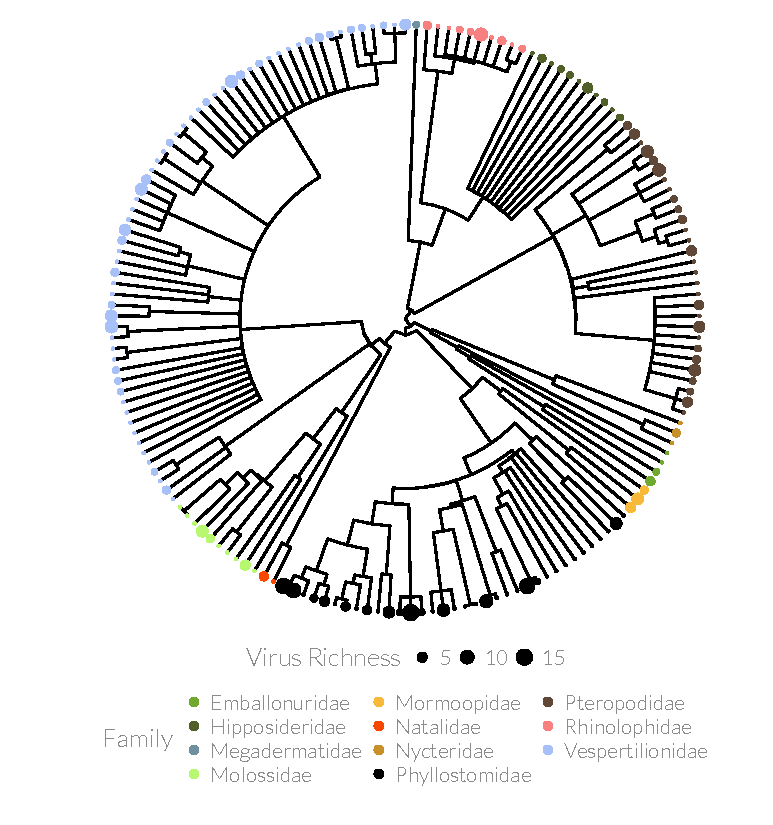
\includegraphics[width=1\textwidth,trim = 0cm 0cm 0cm 0cm]{figures/A-treePlot2-1} 

}

\caption[Pruned alternative phylogeny with dot size showing number of pathogens and colour showing family.]{
Phylogeny from \textcite{jones2005bats} (version 2) pruned to include all species used in the number of subspecies analysis.
Dot size shows the number of known viruses for that species and colour shows family.
Analyses run with this phylogeny gave qualitatively similar results to analyses using the phylogeny from \cite{bininda2007delayed}.
}\label{fig:treePlot2}
\end{figure}


\end{knitrout}





